% !TEX root = BIGALL-Master.tex
\section{Theoretische Grundlagen}
\subsection{Synthese von Nanopartikeln}
	Bei der Herstellung von Nanopartikeln wird zwischen der \glqq bottom-up\grqq - und der \glqq top-down\grqq - Methode unterschieden.
	Bei der \glqq top-down\grqq - Methode wird mit einem Festkörper angefangen, der dann durch verschiedene physikalische Zerkleinerungsmethoden auf eine gewünschte Partikelgröße gebrochen wird.
	Da diese Brüche nicht gleichmäßig stattfinden, eigenen sich diese Methoden nicht um monodisperse Nanokristalle herzustellen.
	Bei der \glqq bottom-up\grqq - Methode wird ein Nanopartikel aus vielen Monomeren zusammengesetzt, bis zur gewünschten Größe.
	Diese Methode kann mit einzelnen Klemmbausteinen verglichen werden, die zu größeren Gebilden zusammengesetzt werden können.
	Da man bei diesem Verfahren viele Parameter hat, die verändert werden können, durch die die Partikeleigenschaften eingestellt werden können, bietet sich das \glqq bottom-up\grqq - Verfahren zur Synthese monodisperser Partikel besser an.
	Parameter die eingestellt werden können sind u.a. Reaktionstemperatur und Dauer, Konzentration der Edukte, Druck oder Lösungsmittel.
	
	Die theoretische Beschreibung der Bildung monodisperser Nanopartikel geht auf Untersuchungen von LaMer und Dinegar zurück.\autocite{Lamer1950}
	Sie zeigten, dass die Bildung
	monodisperser Kolloide eine zeitlich diskrete (nicht kontinuierliche) Keimbildung
	erfordert, gefolgt von einem langsameren kontrollierten Wachstum der existierenden
	Kerne.
	Bei dem Konzept der sog. „schlagartigen Keimbildung“ muss demnach die
	Keimbildung zu einem einzigen Zeitpunkt ausgelöst werden. Weitere
	Keimbildungsereignisse sind auszuschließen. Startend in einer homogenen Phase setzt
	bei Überwindung der Energiebarriere die Keimbildung ein und es resultiert eine
	heterogene Phase unter homogener Nukleation. \autocite{Park2007}
	
	\begin{figure}[H]
		\centering
		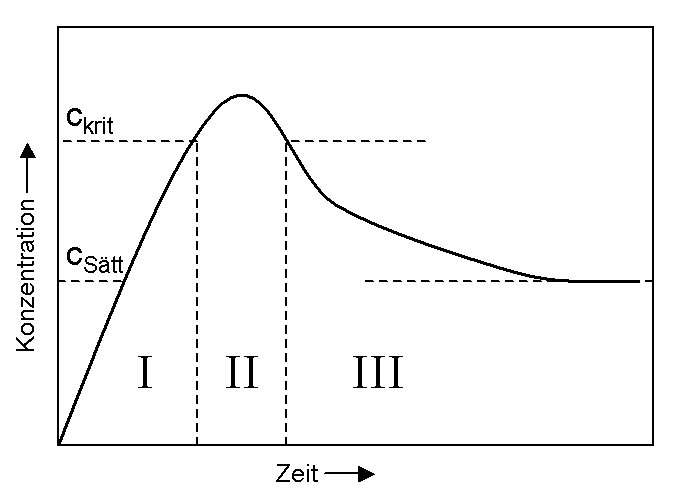
\includegraphics[width=0.6\textwidth]{Bilder/LaMer} 	
		\caption{LaMer-Diagramm: Monomerkonzentration als Funktion der Zeit nach.\autocite{Lamer1950}}
		\label{fig:LaMer}
	\end{figure}

	Im LaMer-Modell existieren 3 Stufen. 
	In Stufe I ist eine kontinuierliche Zunahme der Monomerkonzentration dargestellt.
	Durch die Energiebarriere kommt es auch nach Überschreiten der Sättigungs-Konzentration $C_{Sätt}$ zu keiner Keimbildung.
	Zum Erreichen der Keimbildung in Stufe II muss eine kritische Konzentration $c_{krit}$ überschritten werden.
	Hier werden schlagartig Keime gebildet mit einem kritischen Radius $r_{krit}$, wodurch die Monomerkonzentration wieder unter $c_{krit}$ sinkt, wo dann keine weiteren Keime mehr gebildet werden können.
	Hier wird dann Stufe III erreicht, bei der die Monomere nicht mehr zur Keimbildung, sondern zum Wachstum der Keime genutzt werden, bis ein Gleichgewichtszustand bei der Sättigungskonzentration erreicht wird.
	
%----------------------------------------------
	
	\subsection{Halbleiternanopartikel \& Größenquantisierungseffekt}
	Während Halbleiter als Festkörper eine feste Bandlücke zwischen Valenz- und Leitungsband aufweisen, ist sie bei Nanopartikeln eine von der Partikelgröße abhängige Eigenschaft.
	Allgemein gilt, dass bei kleineren Partikeln die Bandlücke zunimmt.
	\begin{figure}[h]
		\centering
		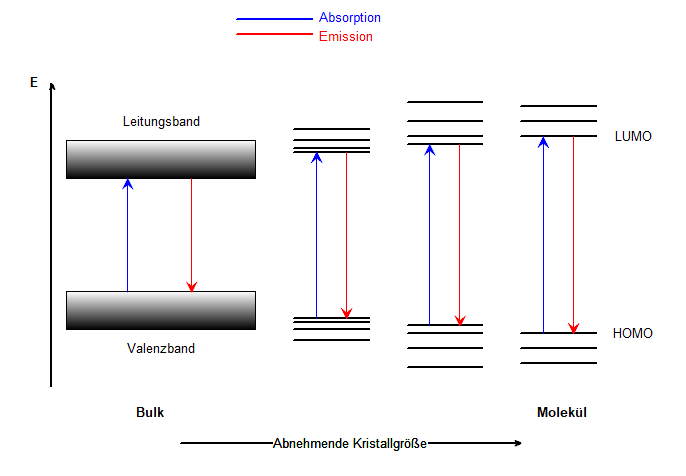
\includegraphics[width=0.6\linewidth]{Bilder/Quantumsizeeffect}
		\caption{Schematische Darstellung der Veränderung der Bandlücke bei abnehmender Kristallgröße.}
		\label{fig:LCAO}
	\end{figure}
	
    Dies lässt sich über 2 Theorien beschreiben. Zum einen auf der Basis des LCAO-Modells (Linear Combination of Atomic Orbitals) bei dem Nanopartikel als große Moleküle gesehen werden, zum anderen auf Basis der Festkörpertheorie, die Nanopartikel als kleine Festkörper beschreibt.
	
	Bei der LCAO-Methode bilden n Atomorbitale, die gleiche Symmetrie und ähnliche Energie besitzen, durch lineare Kombination, n Molekülorbitale. Wird n sehr groß, kommt es zu einer großen Anzahl Energieniveaus, die sehr nahe beieinander liegen, wodurch kontinuierliche Energiebänder entstehen. Bei Isolatoren und Halbleitern gibt es eine Bandlücke zwischen den Bändern, die bei großen Festkörpern, bei denen die Annahme $n \rightarrow \infty$  gilt, zu einer festen Materialeigenschaft führt. Bei Nanopartikeln gilt diese Näherung allerdings nicht mehr, wodurch sich die kontinuierlichen Bänder mit sinkender Anzahl Atomen wieder in diskrete Energieniveaus aufteilen. Dabei vergrößert sich auch die Bandlücke wieder, wie in \cref{fig:LCAO} dargestellt.
	
	Die Festkörpertheorie: Kommt es zur Absorption eines Photons, kommt es zu einem Loch $h^{+}$  im Valenzband und zu einem Elektron $e^{-}$ im Leiterband, die jedoch aufgrund ihrer Polarität, sich nicht frei im Kristall bewegen können und so ein Paar, das Exziton genannt wird, bilden. Der durchschnittliche Abstand von $e^{-}$ und $h^{+}$ wird Exziton-Bohr-Radius genannt. In einem Nanopartikel ist die Bewegung durch die Partikelgrenzen beschränkt, die als Potentialgrenzen wirken, ähnlich des „Teilchen im Kasten“-Modells, bei dem das Potential außerhalb unendlich ist.
	Ist die Partikelgröße kleiner als der Exziton-Bohr-Radius, muss somit die Bandlücke steigen.
	Da ein kristalliner Festkörper kein konstantes Potential aufweist, sondern eher ein periodisch oszillierendes, wird die Effektive-Masse-Näherung angewandt, bei der sowohl $e^{-}$ als auch $h^{+}$ eine effektive Masse zugeordnet wird, die als Maß für Mobilität der Ladungsträger angesehen werden kann. Daraus ergibt sich die BRUS-Formel:
	\begin{equation}
	\label{eq:BRUS}
	E_{NC}=E_{g}+\frac{h^{2}}{8R^{2}}\left( \frac{1}{m^{*}_{e}}+\frac{1}{m^{*}_{h}}\right)-\frac{1,8e^{2}}{4\pi\epsilon_{0}\epsilon_{r}R} 
	\end{equation}
	\begin{multicols}{2}
		\begin{flushleft}
			$E_{NC}$:	Bandlücke des Nanokristalls\\
			$E_{g}$:	Bandlücke des Festkörpers\\
			$h$:		Plank´sches Wirkungsquantum\\
			$R$:		Partikelgröße\\
			$m^{*}_{e}$: Effektive Masse des $e^{-}$\\
			$m^{*}_{h}$: Effektive Masse des $h^{+}$\\
			$\epsilon_{0}$: Permittivität des Vakuums\\
			$\epsilon_{r}$: relative Permittivität\\
			$e$: Elementarladung\\
		\end{flushleft}
	\end{multicols}
	
%-----------------------------------------------------

    \subsection{Metallnanopartikel \& Oberflächenplasmonen}
    
    Metallische Nanopartikel, die kolloidal in Lösung vorliegen, zeigen ein Absorptionsspektrum.
    Dieses ist aber anders als bei Halbleitern nicht auf Elektronenübergänge zwischen quantisierten Energiezuständen einzelner Elektronen, sondern es kommt zu einer kollektiven Anregung eines Elektronenensambles.
    Diese Anregung wird als Oberflächenplasmonenresonanz bezeichnet. \autocite{Mulvaney1996}
    
    Das Phänomen der lokalisierten Oberflächenresonanz (LOPR) entsteht bei der Wechselwirkung von einer elektromagnetischer Welle und frei beweglichen Elektronen eines Metallnanopartikels.\autocite{Hu2006}
    Das periodische elektromagnetische Feld verursacht dabei eine kollektive Oszillation der leitenden Elektronen, wenn die passende Resonanzfrequenz getroffen wird.
    Da die absorbierten Photonen in Phonen des Metallgitters umgewandelt wird, kann kein Emissionsspektrum gemessen werden.
    Für Nanopartikel mit einem Radius $r<<\lambda$, mit $\lambda$ als Wellenlänge, kann in guter Näherung ein, das Partikel durchdringende Feld, als homogen über das gesamte Partikel angenommen werden. \autocite{Xu1999}
    Dadurch kann vereinfacht angenommen werden, dass nur die Dipolanregung zur Extinktion beiträgt und die Dipolaufspaltung als quasistatisch angenommen werden kann.
    
    \begin{figure}
        \centering
        
\includegraphics[width=0.6\linewidth]{Bilder/Muster}
        \caption{Schematische Darstellung der lokalisierten Oberflächenresonanz (LOPR)}
        \label{fig:LOPR}
    \end{figure}
    
    Die plasmonische Resonanzfrequenz ist dabei durch die Permittivität des Metalls, die Größe und Form des Partikels und die Permittivität des umgebenden Mediums. \autocite{Kelly2003,Mock2003}
    Die LOPR-Bande dieser Partikel können sich vom ultravioletten bis in den infraroten Bereich erstrecken. \autocite{Haes2004}
    
    \subsection{Metall-Halbleiter-Nanopartikel}
    Wenn Metallpartikel in Nähe von fluoriszierenden Halbleiter-Nanopartikeln liegen haben diese Einfluss auf die Fluoriszenz dieser.
    Die plasmonischen Metallnanopartikel können als optische Antennen aufgefasst werden, sie können also die zur Anregung der LOPR einfallenden Strahlung im Nahfeld lokalisieren. 
    Je nach Abstand zwischen beiden kann es sowohl zu Fluoriszenzverstärkung als auch zu Fluoriszenzauslöschung kommen. \autocite{Kulakovich2002,Viste2010}
    
    Die Verstärkung kann hauptsächlich auf den Anstieg der Anregungsrate im Fluorophor zurückgeführt werden.\autocite{Chen2008}
    Eine Verstärkung kann durch die chemische Kupplung mit definierten Abstand von plasmonischen Partikeln an die Oberfläche der Halbleiter-Nanopartikel.\autocite{Lee2004}
    
    Die Auslöschung wird durch sehr geringe Abstände oder eine direkte chemische Bindung verursacht.\autocite{Costi2010}
    Hier kommt es an der Grenzfläche zur Ladungstrennung, bei dem ein Elektron aus dem Leitungsband des Halbleiters in die Metalldomäne übertragen wird.
    Dadurch erhöht sich die Menge an strahlungsfreier Relaxation.
    
    
    \subsection{Nanopartikelbasierte Gele}
    
    Allgemein sind Gele Systeme aus mindestens zwei Komponenten, wobei eines ein festes dreidimensionales Netzwerk bildet und von einer Flüssigkeit oder einem Gas ausgefüllt ist. \autocite{Aleman2007}
    
    Der klassische Bildungsmechanismus folgt meist dem Sol-Gel-Verfahren. \autocite{Ziegler2017}
    Dabei wird aus einem flüssigen System über stufenweise Umwandlungen von Vorstufen ein Sol gebildet woraus anschließend ein Gel entsteht. \autocite{Aleman2007}
    Diese Umwandlungen sind meist Polymerisationsreaktionen oder bei anorganischen, oxidschen Gelen Kondensationsreaktionen. 
    Da bei diesen Reaktionen das Material, das das Sol und später das Netzwerk bildet, das gleiche ist, wie das verknüpfende, können diese Prozesse nur für spezielle Materialien durchgeführt werden.
    
    Da viele Eigenschaften von Nanopartikeln form- und größenabhängig sind, diese aber bei diesem klassischen Ansatz nur schwer bis gar nicht einstellbar sind, eignet er sich für die Gelierung von Nanopartikeln nicht gut.
    
    Dieses Problem konnte erstmals in der Arbeit von Brock und Monahan 2004 umgangen werden, durch kontrollierte Destabilisierung der Nanopartikel. \autocite{Mohanan2004,Mohanan2005}
    Diese Destabilisierung erfolgt durch Zugabe eines Oxidationsmittels in eine Lösung von ligandenstabilisierten Nanopartikeln.
    Durch diese Zugabe reagieren Teile der Liganden miteinander, wodurch es zu offenen Stellen an der Oberfläche der Nanopartikel kommt, an denen die Partikel dann aggregieren können.
    Neben diesem Ansatz sind auch andere Gelierungsstrategien bekannt, die in \cref{fig:Destabilisierung} gezeigt sind.
    
    \begin{figure}[H]
        \centering
        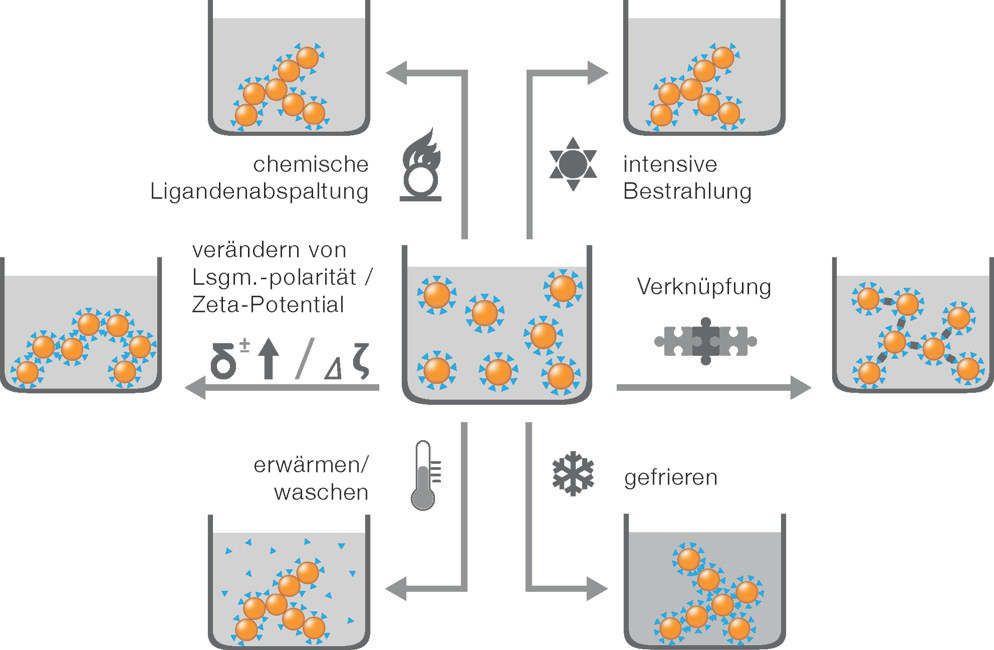
\includegraphics[width=0.6\linewidth]{Bilder/Gelierung.png}
        \caption{Strategien für die kontrollierte Destabilisierung von vorab gebildeten kolloidalen Lösungen.\autocite{Aleman2007}}
        \label{fig:Destabilisierung}
    \end{figure}
    
    Auf diese Weise können auch metallische Nanopartikel zu Gelen weiterverarbeitet werden. \autocite{Bigall2009}
    Diese zeigen vielversprechende Eigenschaften bei verschiedenen elektrokatalytischen Prozessen wie Alkoholoxidation, Sauerstoffreduktionsreaktion und Sauerstoffentwicklungsreaktion. \autocite{Cai2018,Shi2018,Zhu2016,Shi2017,Wang2019}
    Edelmetall-Nanostrukturen weisen einzigartige optische Eigenschaften auf, die eine Kopplung zwischen den kollektiven Oberflächenelektronenoszillationen und dem einfallenden elektromagnetischen Feld ermöglichen und so ein dramatisch verstärktes lokales elektrisches Feld für eine oberflächenverstärkte Raman-Streuung ergeben. \autocite{Linic2015,Gao2016}

    
    \subsection{Metall-Halbleiter-Gele}
    Die meisten Untersuchungen von Gelen, die Halbleiter und Metallnanopartikel enthalten, sind Gele mit gemischter Zusammensetzung, bei der Halbleitergele mit Metallnanopartikel wie Gold oder Silber modifiziert werden.\autocite{Nahar2015,Lesnyak2011} 
    Hier können Emissionen beobachtet werden mit Zerfallsraten,  die beim reinen Halbleitergel nicht beobachtet werden können, was auf die Erzeugung alternativer Strahlungszerfälle hinweist. \autocite{Nahar2015}
    Gleichzeitig können bei höheren Raten an Metallpartikeln die Fluoriszenz ausgelöscht werden. \autocite{Lesnyak2011}